% Options for packages loaded elsewhere
\PassOptionsToPackage{unicode}{hyperref}
\PassOptionsToPackage{hyphens}{url}
%
\documentclass[
]{article}
\usepackage{amsmath,amssymb}
\usepackage{iftex}
\ifPDFTeX
  \usepackage[T1]{fontenc}
  \usepackage[utf8]{inputenc}
  \usepackage{textcomp} % provide euro and other symbols
\else % if luatex or xetex
  \usepackage{unicode-math} % this also loads fontspec
  \defaultfontfeatures{Scale=MatchLowercase}
  \defaultfontfeatures[\rmfamily]{Ligatures=TeX,Scale=1}
\fi
\usepackage{lmodern}
\ifPDFTeX\else
  % xetex/luatex font selection
\fi
% Use upquote if available, for straight quotes in verbatim environments
\IfFileExists{upquote.sty}{\usepackage{upquote}}{}
\IfFileExists{microtype.sty}{% use microtype if available
  \usepackage[]{microtype}
  \UseMicrotypeSet[protrusion]{basicmath} % disable protrusion for tt fonts
}{}
\makeatletter
\@ifundefined{KOMAClassName}{% if non-KOMA class
  \IfFileExists{parskip.sty}{%
    \usepackage{parskip}
  }{% else
    \setlength{\parindent}{0pt}
    \setlength{\parskip}{6pt plus 2pt minus 1pt}}
}{% if KOMA class
  \KOMAoptions{parskip=half}}
\makeatother
\usepackage{xcolor}
\usepackage{color}
\usepackage{fancyvrb}
\newcommand{\VerbBar}{|}
\newcommand{\VERB}{\Verb[commandchars=\\\{\}]}
\DefineVerbatimEnvironment{Highlighting}{Verbatim}{commandchars=\\\{\}}
% Add ',fontsize=\small' for more characters per line
\newenvironment{Shaded}{}{}
\newcommand{\AlertTok}[1]{\textcolor[rgb]{1.00,0.00,0.00}{\textbf{#1}}}
\newcommand{\AnnotationTok}[1]{\textcolor[rgb]{0.38,0.63,0.69}{\textbf{\textit{#1}}}}
\newcommand{\AttributeTok}[1]{\textcolor[rgb]{0.49,0.56,0.16}{#1}}
\newcommand{\BaseNTok}[1]{\textcolor[rgb]{0.25,0.63,0.44}{#1}}
\newcommand{\BuiltInTok}[1]{\textcolor[rgb]{0.00,0.50,0.00}{#1}}
\newcommand{\CharTok}[1]{\textcolor[rgb]{0.25,0.44,0.63}{#1}}
\newcommand{\CommentTok}[1]{\textcolor[rgb]{0.38,0.63,0.69}{\textit{#1}}}
\newcommand{\CommentVarTok}[1]{\textcolor[rgb]{0.38,0.63,0.69}{\textbf{\textit{#1}}}}
\newcommand{\ConstantTok}[1]{\textcolor[rgb]{0.53,0.00,0.00}{#1}}
\newcommand{\ControlFlowTok}[1]{\textcolor[rgb]{0.00,0.44,0.13}{\textbf{#1}}}
\newcommand{\DataTypeTok}[1]{\textcolor[rgb]{0.56,0.13,0.00}{#1}}
\newcommand{\DecValTok}[1]{\textcolor[rgb]{0.25,0.63,0.44}{#1}}
\newcommand{\DocumentationTok}[1]{\textcolor[rgb]{0.73,0.13,0.13}{\textit{#1}}}
\newcommand{\ErrorTok}[1]{\textcolor[rgb]{1.00,0.00,0.00}{\textbf{#1}}}
\newcommand{\ExtensionTok}[1]{#1}
\newcommand{\FloatTok}[1]{\textcolor[rgb]{0.25,0.63,0.44}{#1}}
\newcommand{\FunctionTok}[1]{\textcolor[rgb]{0.02,0.16,0.49}{#1}}
\newcommand{\ImportTok}[1]{\textcolor[rgb]{0.00,0.50,0.00}{\textbf{#1}}}
\newcommand{\InformationTok}[1]{\textcolor[rgb]{0.38,0.63,0.69}{\textbf{\textit{#1}}}}
\newcommand{\KeywordTok}[1]{\textcolor[rgb]{0.00,0.44,0.13}{\textbf{#1}}}
\newcommand{\NormalTok}[1]{#1}
\newcommand{\OperatorTok}[1]{\textcolor[rgb]{0.40,0.40,0.40}{#1}}
\newcommand{\OtherTok}[1]{\textcolor[rgb]{0.00,0.44,0.13}{#1}}
\newcommand{\PreprocessorTok}[1]{\textcolor[rgb]{0.74,0.48,0.00}{#1}}
\newcommand{\RegionMarkerTok}[1]{#1}
\newcommand{\SpecialCharTok}[1]{\textcolor[rgb]{0.25,0.44,0.63}{#1}}
\newcommand{\SpecialStringTok}[1]{\textcolor[rgb]{0.73,0.40,0.53}{#1}}
\newcommand{\StringTok}[1]{\textcolor[rgb]{0.25,0.44,0.63}{#1}}
\newcommand{\VariableTok}[1]{\textcolor[rgb]{0.10,0.09,0.49}{#1}}
\newcommand{\VerbatimStringTok}[1]{\textcolor[rgb]{0.25,0.44,0.63}{#1}}
\newcommand{\WarningTok}[1]{\textcolor[rgb]{0.38,0.63,0.69}{\textbf{\textit{#1}}}}
\usepackage{graphicx}
\makeatletter
\def\maxwidth{\ifdim\Gin@nat@width>\linewidth\linewidth\else\Gin@nat@width\fi}
\def\maxheight{\ifdim\Gin@nat@height>\textheight\textheight\else\Gin@nat@height\fi}
\makeatother
% Scale images if necessary, so that they will not overflow the page
% margins by default, and it is still possible to overwrite the defaults
% using explicit options in \includegraphics[width, height, ...]{}
\setkeys{Gin}{width=\maxwidth,height=\maxheight,keepaspectratio}
% Set default figure placement to htbp
\makeatletter
\def\fps@figure{htbp}
\makeatother
\setlength{\emergencystretch}{3em} % prevent overfull lines
\providecommand{\tightlist}{%
  \setlength{\itemsep}{0pt}\setlength{\parskip}{0pt}}
\setcounter{secnumdepth}{-\maxdimen} % remove section numbering
\ifLuaTeX
  \usepackage{selnolig}  % disable illegal ligatures
\fi
\IfFileExists{bookmark.sty}{\usepackage{bookmark}}{\usepackage{hyperref}}
\IfFileExists{xurl.sty}{\usepackage{xurl}}{} % add URL line breaks if available
\urlstyle{same}
\hypersetup{
  hidelinks,
  pdfcreator={LaTeX via pandoc}}

\author{}
\date{}

\begin{document}

\hypertarget{frequency-domain-filtering}{%
\section{Frequency Domain Filtering}\label{frequency-domain-filtering}}

\hypertarget{introduction}{%
\section{Introduction}\label{introduction}}

In this lab, we delved into the frequency domain filtering technique
while also comparing it with spatial filtering. Specifically, we first
investigate the Sobel filtering in both the spatial domain and the
frequency domain. Next, we perform a Butterworth notch filtering
individually in the frequency domain, which involves a great deal of
steps needed to pay attention to.

\hypertarget{sobel-filtering}{%
\section{Sobel Filtering}\label{sobel-filtering}}

\hypertarget{in-spatial-domain}{%
\subsection{In Spatial Domain}\label{in-spatial-domain}}

To perform Sobel filtering to an image in the spatial domain, we can
directly perform 2D convolution.

First, flip the Sobel kernel using the following code:

\begin{Shaded}
\begin{Highlighting}[]
\NormalTok{kernel }\OperatorTok{=}\NormalTok{ np.flipud(np.fliplr(kernel))}
\end{Highlighting}
\end{Shaded}

This step is really often omitted because a spatial kernel is usually
symmetric, however, this is not the case for a Sobel kernel, which is a
kernel in the form of this:

\begin{bmatrix}
-1&0&1\\
-2&0&2\\
-1&0&1
\end{bmatrix}

As we can see, this kernel is not symmetric. Thus, the flipping is
necessary in this case; if we don't perform this step, the output image
can have a different changing direction of the texture, as shown in
Figure todo.

Next, multiply, add, and slide the kernel, and then we can obtain the
desired image filtered by the Sobel spatial kernel.

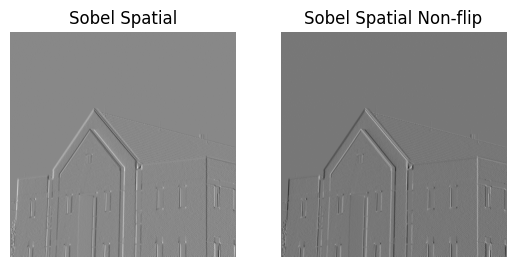
\includegraphics{D:/Tangent/SUSTech/大三下/课程资料/DIP/Lab/lab repo/Lab5/report/assets/sobel_spatial.png}

The code for spatial filtering is shown below:

\begin{Shaded}
\begin{Highlighting}[]
\KeywordTok{def}\NormalTok{ sobel\_spatial(img: np.ndarray, flipping }\OperatorTok{=} \VariableTok{True}\NormalTok{):}
\NormalTok{    sobel\_y }\OperatorTok{=}\NormalTok{ np.array([[}\OperatorTok{{-}}\DecValTok{1}\NormalTok{, }\DecValTok{0}\NormalTok{, }\DecValTok{1}\NormalTok{], [}\OperatorTok{{-}}\DecValTok{2}\NormalTok{, }\DecValTok{0}\NormalTok{, }\DecValTok{2}\NormalTok{], [}\OperatorTok{{-}}\DecValTok{1}\NormalTok{, }\DecValTok{0}\NormalTok{, }\DecValTok{1}\NormalTok{]])}
    \ControlFlowTok{if}\NormalTok{ flipping:}
\NormalTok{        mask\_y }\OperatorTok{=}\NormalTok{ conv2d(img, sobel\_y, stride}\OperatorTok{=}\DecValTok{1}\NormalTok{, padding}\OperatorTok{=}\DecValTok{1}\NormalTok{,flipping}\OperatorTok{=}\VariableTok{True}\NormalTok{)}
    \ControlFlowTok{else}\NormalTok{:}
\NormalTok{        mask\_y }\OperatorTok{=}\NormalTok{ conv2d(img, sobel\_y, stride}\OperatorTok{=}\DecValTok{1}\NormalTok{, padding}\OperatorTok{=}\DecValTok{1}\NormalTok{,flipping}\OperatorTok{=}\VariableTok{False}\NormalTok{)}
    \ControlFlowTok{return}\NormalTok{ mask\_y}

\KeywordTok{def}\NormalTok{ conv2d(img: np.ndarray, kernel: np.ndarray, stride: }\BuiltInTok{int} \OperatorTok{=} \DecValTok{0}\NormalTok{, padding: }\BuiltInTok{int} \OperatorTok{=} \DecValTok{0}\NormalTok{, flipping }\OperatorTok{=}\VariableTok{True}\NormalTok{) }\OperatorTok{{-}\textgreater{}}\NormalTok{ np.ndarray:}
\NormalTok{    temp }\OperatorTok{=}\NormalTok{ np.pad(img, padding, mode}\OperatorTok{=}\StringTok{\textquotesingle{}reflect\textquotesingle{}}\NormalTok{)}
    \ControlFlowTok{if}\NormalTok{ flipping:}
\NormalTok{        kernel }\OperatorTok{=}\NormalTok{ np.flipud(np.fliplr(kernel))}
\NormalTok{    out\_img }\OperatorTok{=}\NormalTok{ np.zeros(img.shape)}
    \ControlFlowTok{for}\NormalTok{ i }\KeywordTok{in} \BuiltInTok{range}\NormalTok{(}\DecValTok{0}\NormalTok{, img.shape[}\DecValTok{0}\NormalTok{], stride):}
        \ControlFlowTok{for}\NormalTok{ j }\KeywordTok{in} \BuiltInTok{range}\NormalTok{(}\DecValTok{0}\NormalTok{, img.shape[}\DecValTok{1}\NormalTok{], stride):}
\NormalTok{            out\_img[i, j] }\OperatorTok{=}\NormalTok{ np.}\BuiltInTok{sum}\NormalTok{(temp[i:i}\OperatorTok{+}\NormalTok{kernel.shape[}\DecValTok{0}\NormalTok{], j:j}\OperatorTok{+}\NormalTok{kernel.shape[}\DecValTok{1}\NormalTok{]] }\OperatorTok{*}\NormalTok{ kernel)}
    \ControlFlowTok{return}\NormalTok{ out\_img}
\end{Highlighting}
\end{Shaded}

\hypertarget{in-frequency-domain}{%
\subsection{In Frequency Domain}\label{in-frequency-domain}}

Performing frequency domain filtering is much trickier than spatial
domain. Since we can only perform Discrete Fourier Transform (DFT) to an
image or kernel in a digital computer, and the spectrum of DFT (or its
fast implementation version: FFT) is sampled from a full Fourier
spectrum, which can cause wrap-around error if we don't pad zeros to the
image and the kernel before doing frequency domain filtering.

First, we need to pad the image and the kernel to a suitable size, which
means if the image is of size \(H\times W\), and the kernel is of size
\(m\times n\), then we need to pad both the image and the kernel to size
\((H+m-1)\times (W+n-1)\). Note that, we pad zeros in the direction
along the positive direction of two axes, which can preserve the
position of the image after filtering.

Then, do FFT2 to both the padded image and the padded kernel, and
multiply them in the frequency domain.

Next, IFFT2 is performed, and the imaginary part of the image is set to
zero to deal with the parasitic imaginary part.

Finally, crop the image to the original size.

The code for the frequency domain filtering is shown below:

\begin{Shaded}
\begin{Highlighting}[]
\KeywordTok{def}\NormalTok{ sobel\_freq(img: np.ndarray):}
\NormalTok{    sobel }\OperatorTok{=}\NormalTok{ pad\_sobel(}\BuiltInTok{int}\NormalTok{(img.shape[}\DecValTok{0}\NormalTok{]}\OperatorTok{{-}}\DecValTok{1}\NormalTok{), }\BuiltInTok{int}\NormalTok{(img.shape[}\DecValTok{1}\NormalTok{])}\OperatorTok{{-}}\DecValTok{1}\NormalTok{)}
\NormalTok{    img\_pad }\OperatorTok{=}\NormalTok{ np.pad(img, ((}\DecValTok{0}\NormalTok{, }\DecValTok{2}\NormalTok{), (}\DecValTok{0}\NormalTok{, }\DecValTok{2}\NormalTok{)), mode}\OperatorTok{=}\StringTok{\textquotesingle{}constant\textquotesingle{}}\NormalTok{, constant\_values}\OperatorTok{=}\DecValTok{0}\NormalTok{)}
\NormalTok{    X\_img }\OperatorTok{=}\NormalTok{ np.fft.fft2(img\_pad)}
\NormalTok{    H\_sobel }\OperatorTok{=}\NormalTok{ np.fft.fft2(sobel)}
\NormalTok{    Y\_img }\OperatorTok{=}\NormalTok{ X\_img }\OperatorTok{*}\NormalTok{ H\_sobel}
\NormalTok{    y\_img }\OperatorTok{=}\NormalTok{ np.fft.ifft2(Y\_img)}
\NormalTok{    y\_img }\OperatorTok{=}\NormalTok{ np.real(y\_img)}
\NormalTok{    y\_img }\OperatorTok{=}\NormalTok{ y\_img[}\DecValTok{0}\NormalTok{:}\OperatorTok{{-}}\DecValTok{2}\NormalTok{, }\DecValTok{0}\NormalTok{:}\OperatorTok{{-}}\DecValTok{2}\NormalTok{]}
\NormalTok{    plt.figure()}
\NormalTok{    plt.subplot(}\DecValTok{1}\NormalTok{,}\DecValTok{2}\NormalTok{,}\DecValTok{1}\NormalTok{)}
\NormalTok{    plt.imshow(sobel, cmap}\OperatorTok{=}\StringTok{\textquotesingle{}gray\textquotesingle{}}\NormalTok{)}
\NormalTok{    plt.axis(}\StringTok{\textquotesingle{}off\textquotesingle{}}\NormalTok{)}
\NormalTok{    plt.title(}\StringTok{\textquotesingle{}Sobel Filter\textquotesingle{}}\NormalTok{)}
\NormalTok{    plt.subplot(}\DecValTok{1}\NormalTok{,}\DecValTok{2}\NormalTok{,}\DecValTok{2}\NormalTok{)}
\NormalTok{    plt.imshow(img\_pad, cmap}\OperatorTok{=}\StringTok{\textquotesingle{}gray\textquotesingle{}}\NormalTok{)}
\NormalTok{    plt.axis(}\StringTok{\textquotesingle{}off\textquotesingle{}}\NormalTok{)}
\NormalTok{    plt.title(}\StringTok{\textquotesingle{}Padded Image\textquotesingle{}}\NormalTok{)}
\NormalTok{    plt.show()}
    \ControlFlowTok{return}\NormalTok{ y\_img}

\KeywordTok{def}\NormalTok{ pad\_sobel(padding\_x: }\BuiltInTok{int} \OperatorTok{=} \DecValTok{1}\NormalTok{, padding\_y: }\BuiltInTok{int} \OperatorTok{=} \DecValTok{1}\NormalTok{):}
\NormalTok{    sobel\_y }\OperatorTok{=}\NormalTok{ np.array([[}\OperatorTok{{-}}\DecValTok{1}\NormalTok{, }\DecValTok{0}\NormalTok{, }\DecValTok{1}\NormalTok{], [}\OperatorTok{{-}}\DecValTok{2}\NormalTok{, }\DecValTok{0}\NormalTok{, }\DecValTok{2}\NormalTok{], [}\OperatorTok{{-}}\DecValTok{1}\NormalTok{, }\DecValTok{0}\NormalTok{, }\DecValTok{1}\NormalTok{]])}
\NormalTok{    sobel\_y }\OperatorTok{=}\NormalTok{ np.pad(sobel\_y, ((}\DecValTok{0}\NormalTok{, padding\_x), }\OperatorTok{\textbackslash{}}
\NormalTok{                    (}\DecValTok{0}\NormalTok{, padding\_y)), mode}\OperatorTok{=}\StringTok{\textquotesingle{}constant\textquotesingle{}}\NormalTok{, constant\_values}\OperatorTok{=}\DecValTok{0}\NormalTok{)}
    \ControlFlowTok{return}\NormalTok{ sobel\_y}
\end{Highlighting}
\end{Shaded}

The spatial and frequency domain filtering results are almost the same
as shown in Figure todo.

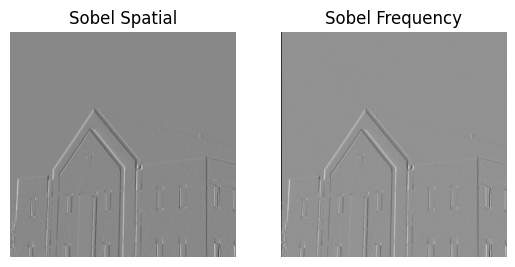
\includegraphics{D:/Tangent/SUSTech/大三下/课程资料/DIP/Lab/lab repo/Lab5/report/assets/sobel_spatial_freq.png}

Except for the black edge in the frequency domain filtered results,
which is because we pad the image in spatial convolution in
\texttt{reflect} mode.

\begin{Shaded}
\begin{Highlighting}[]
\KeywordTok{def}\NormalTok{ conv2d(...):}
\NormalTok{    ...}
\NormalTok{	temp }\OperatorTok{=}\NormalTok{ np.pad(img, padding, mode}\OperatorTok{=}\StringTok{\textquotesingle{}reflect\textquotesingle{}}\NormalTok{)}
\NormalTok{	...}
\end{Highlighting}
\end{Shaded}

\hypertarget{remarks}{%
\subsection{Remarks}\label{remarks}}

In the textbook, the author performs the frequency domain filtering
differently as shown below:

\begin{quote}
Generating \(H(u,v)\)

\begin{enumerate}
\def\labelenumi{\arabic{enumi}.}
\item
  Multiply \(h_p(x,y)\) by \((-1)^{x+y} \) to center the frequency
  domain filter
\item
  Compute the forward DFT of the result in (1)
\item
  Set the real part of the resulting DFT to 0 to account for parasitic
  real parts
\item
  Multiply the result by \((-1)^{u+v} \) which is implicit when
  \( h_p(x,y) \) was moved to the center of \( H(u,v) \).
\end{enumerate}
\end{quote}

The first step, centering the kernel, is not necessary for computation
but is good for visualization of the spectrum.

In the fourth step, which multiplies the frequency spectrum of
\(h_p(x, y)\) with \((-1)^{u+v}\) , the author intends to move the
spatial kernel which is padded to the center back to the corner. The
author padded the kernel to the center first because making the padded
kernel odd-symmetric can have a special effect of preserving the image
phase, which is important for image information preservation.

But I still doubt this step is necessary if I don't need to pad the
kernel to center at the beginning.

\hypertarget{butterworth-notch-filter}{%
\section{Butterworth Notch Filter}\label{butterworth-notch-filter}}

Sometimes, there is some noise in the image, which exhibits a periodic
fashion; we can use a Butterworth notch filter to deal with this
situation.

As shown in Figure todo, we notice a periodic grid pattern in the image.
If we do an FFT2 to this image, the magnitude spectrum shows eight
bright spots separated around the central bright pattern. And those
eight bright spots are the noise.

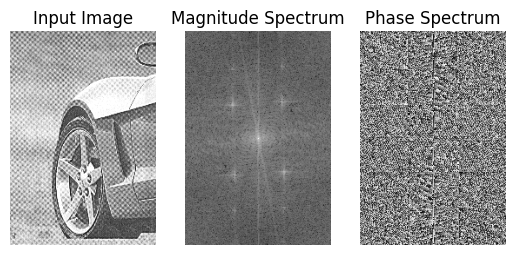
\includegraphics{D:/Tangent/SUSTech/大三下/课程资料/DIP/Lab/lab repo/Lab5/report/assets/17-52-49.png}

To filter out this noise, we need to use a notch filter because no
matter whether it is a low pass filter, high pass filter, or bandpass
filter, all centered at the middle of the spectrum, it is impossible to
filter out the noise without affecting the main information of the
image.

Using a Butterworth filter instead of an ideal filter is because an
ideal notch filter can impose a significant ring effect, which can be
eliminated by choosing a Butterworth notch filter.

The frequency spectrum of this filter is shown in Figure todo.

The result after filtering is shown in Figure todo.

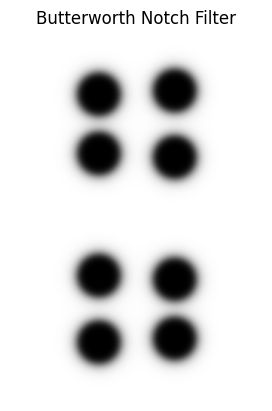
\includegraphics{D:/Tangent/SUSTech/大三下/课程资料/DIP/Lab/lab repo/Lab5/report/assets/butterworth_notch.png}

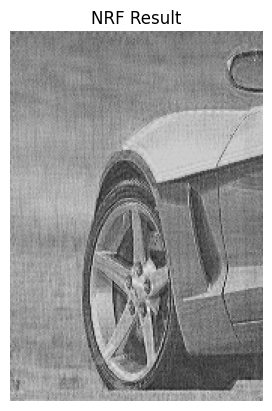
\includegraphics{D:/Tangent/SUSTech/大三下/课程资料/DIP/Lab/lab repo/Lab5/report/assets/nrf.png}

If we do the FFT2 to the filtered result (Figure todo), we can notice
that the noise in the spectrum has been filtered out.

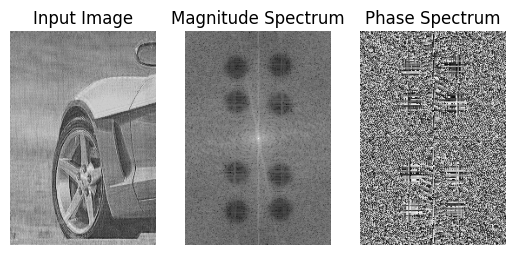
\includegraphics{D:/Tangent/SUSTech/大三下/课程资料/DIP/Lab/lab repo/Lab5/report/assets/18-06-38.png}

The code performing Butterworth notch filter is shown below:

\begin{Shaded}
\begin{Highlighting}[]
\KeywordTok{def}\NormalTok{ butter\_notch(D0k: }\BuiltInTok{list}\NormalTok{, img: np.ndarray, uk: }\BuiltInTok{list}\NormalTok{, vk: }\BuiltInTok{list}\NormalTok{ ,order: }\BuiltInTok{int} \OperatorTok{=} \DecValTok{4}\NormalTok{, scale }\OperatorTok{=} \VariableTok{True}\NormalTok{):}
    \ControlFlowTok{assert} \BuiltInTok{len}\NormalTok{(D0k) }\OperatorTok{==} \BuiltInTok{len}\NormalTok{(uk) }\OperatorTok{==} \BuiltInTok{len}\NormalTok{(vk), }\StringTok{\textquotesingle{}Invalid input. \# of D0k, uk, vk should be the same.\textquotesingle{}}
\NormalTok{    img\_pad }\OperatorTok{=}\NormalTok{ np.pad(img, ((}\DecValTok{0}\NormalTok{,img.shape[}\DecValTok{0}\NormalTok{]), (}\DecValTok{0}\NormalTok{,img.shape[}\DecValTok{1}\NormalTok{])), mode}\OperatorTok{=} \StringTok{\textquotesingle{}constant\textquotesingle{}}\NormalTok{, constant\_values}\OperatorTok{=}\DecValTok{0}\NormalTok{)}
\NormalTok{    X\_img }\OperatorTok{=}\NormalTok{ np.fft.fft2(img\_pad)}
\NormalTok{    X\_img }\OperatorTok{=}\NormalTok{ np.fft.fftshift(X\_img)}

\NormalTok{    uu,vv }\OperatorTok{=}\NormalTok{ np.ogrid[}\DecValTok{0}\NormalTok{:X\_img.shape[}\DecValTok{0}\NormalTok{], }\DecValTok{0}\NormalTok{:X\_img.shape[}\DecValTok{1}\NormalTok{]]}

\NormalTok{    Dk }\OperatorTok{=}\NormalTok{ []}
\NormalTok{    D\_k }\OperatorTok{=}\NormalTok{ []}
\NormalTok{    H }\OperatorTok{=}\NormalTok{ np.ones(X\_img.shape)}

    \ControlFlowTok{if}\NormalTok{ scale:}
\NormalTok{        uk }\OperatorTok{=}\NormalTok{ [u }\OperatorTok{*}\NormalTok{ X\_img.shape[}\DecValTok{0}\NormalTok{] }\ControlFlowTok{for}\NormalTok{ u }\KeywordTok{in}\NormalTok{ uk]}
\NormalTok{        vk }\OperatorTok{=}\NormalTok{ [v }\OperatorTok{*}\NormalTok{ X\_img.shape[}\DecValTok{1}\NormalTok{] }\ControlFlowTok{for}\NormalTok{ v }\KeywordTok{in}\NormalTok{ vk]}

    \ControlFlowTok{for}\NormalTok{ k }\KeywordTok{in} \BuiltInTok{range}\NormalTok{(}\BuiltInTok{len}\NormalTok{(D0k)):}
\NormalTok{        dk }\OperatorTok{=}\NormalTok{ np.sqrt((uu}\OperatorTok{{-}}\NormalTok{uk[k])}\OperatorTok{**}\DecValTok{2} \OperatorTok{+}\NormalTok{ (vv }\OperatorTok{{-}}\NormalTok{vk[k])}\OperatorTok{**}\DecValTok{2}\NormalTok{)}
\NormalTok{        d\_k }\OperatorTok{=}\NormalTok{ np.sqrt((uu}\OperatorTok{{-}}\NormalTok{(X\_img.shape[}\DecValTok{0}\NormalTok{]}\OperatorTok{{-}}\NormalTok{uk[k]))}\OperatorTok{**}\DecValTok{2} \OperatorTok{+}\NormalTok{ (vv }\OperatorTok{{-}}\NormalTok{ (X\_img.shape[}\DecValTok{1}\NormalTok{]}\OperatorTok{{-}}\NormalTok{vk[k]))}\OperatorTok{**}\DecValTok{2}\NormalTok{)}
\NormalTok{        H }\OperatorTok{=}\NormalTok{ H }\OperatorTok{*}\NormalTok{ (}\DecValTok{1}\OperatorTok{/}\NormalTok{(}\DecValTok{1}\OperatorTok{+}\NormalTok{(D0k[k]}\OperatorTok{/}\NormalTok{dk)}\OperatorTok{**}\NormalTok{(}\DecValTok{2}\OperatorTok{*}\NormalTok{order))) }\OperatorTok{*}\NormalTok{ (}\DecValTok{1}\OperatorTok{/}\NormalTok{(}\DecValTok{1}\OperatorTok{+}\NormalTok{(D0k[k]}\OperatorTok{/}\NormalTok{d\_k)}\OperatorTok{**}\NormalTok{(}\DecValTok{2}\OperatorTok{*}\NormalTok{order)))}
\NormalTok{    Y\_img }\OperatorTok{=}\NormalTok{ X\_img }\OperatorTok{*}\NormalTok{ H}
\NormalTok{    Y\_img }\OperatorTok{=}\NormalTok{ np.fft.ifftshift(Y\_img)}
\NormalTok{    y\_img }\OperatorTok{=}\NormalTok{ np.fft.ifft2(Y\_img)}
\NormalTok{    y\_img }\OperatorTok{=}\NormalTok{ np.real(y\_img)}
\NormalTok{    y\_img }\OperatorTok{=}\NormalTok{ y\_img[}\DecValTok{0}\NormalTok{:img.shape[}\DecValTok{0}\NormalTok{], }\DecValTok{0}\NormalTok{:img.shape[}\DecValTok{1}\NormalTok{]]}
    \ControlFlowTok{return}\NormalTok{ y\_img}
\end{Highlighting}
\end{Shaded}

\hypertarget{remarks-2}{%
\subsection{Remarks}\label{remarks-2}}

In the definition of the function performing Butterworth notch filter,
there are several parameters we need to determine beforehands.

\begin{Shaded}
\begin{Highlighting}[]
\KeywordTok{def}\NormalTok{ butter\_notch(D0k: }\BuiltInTok{list}\NormalTok{, img: np.ndarray, uk: }\BuiltInTok{list}\NormalTok{, vk: }\BuiltInTok{list}\NormalTok{ ,order: }\BuiltInTok{int} \OperatorTok{=} \DecValTok{4}\NormalTok{, scale }\OperatorTok{=} \VariableTok{True}\NormalTok{):}
\end{Highlighting}
\end{Shaded}

\begin{itemize}
\item
  \texttt{D0k}: a list of length \texttt{k}, every element in the list
  is the radius of each notch in the spectrum.
\item
  \texttt{uk}, \texttt{vk}: both of length \texttt{k}, \((uk, vk)\) is
  the center of each notch
\item
  \texttt{order}: order of the Butterworth filter
\item
  \texttt{scale}: if \texttt{True}, it means that the input \((uk, vk)\)
  is expressed in scale(i.e. \(uk/img.shape[0]\) and
  \(vk/ung,shape[1]\))
\end{itemize}

For \texttt{D0k}, we should not set it too large or too small. If it is
too large, noise and the useful information in the image will be
filtered out. If it is too small, we cannot effectively filter out the
noise. I chose D0k=30(pixels) and found that it works pretty well.

After setting \texttt{scale=True}, we can find the \texttt{uk} and
\texttt{vk} by using the snipping tool which can help us to determine
the position of the bright spot as shown in Figure todo.

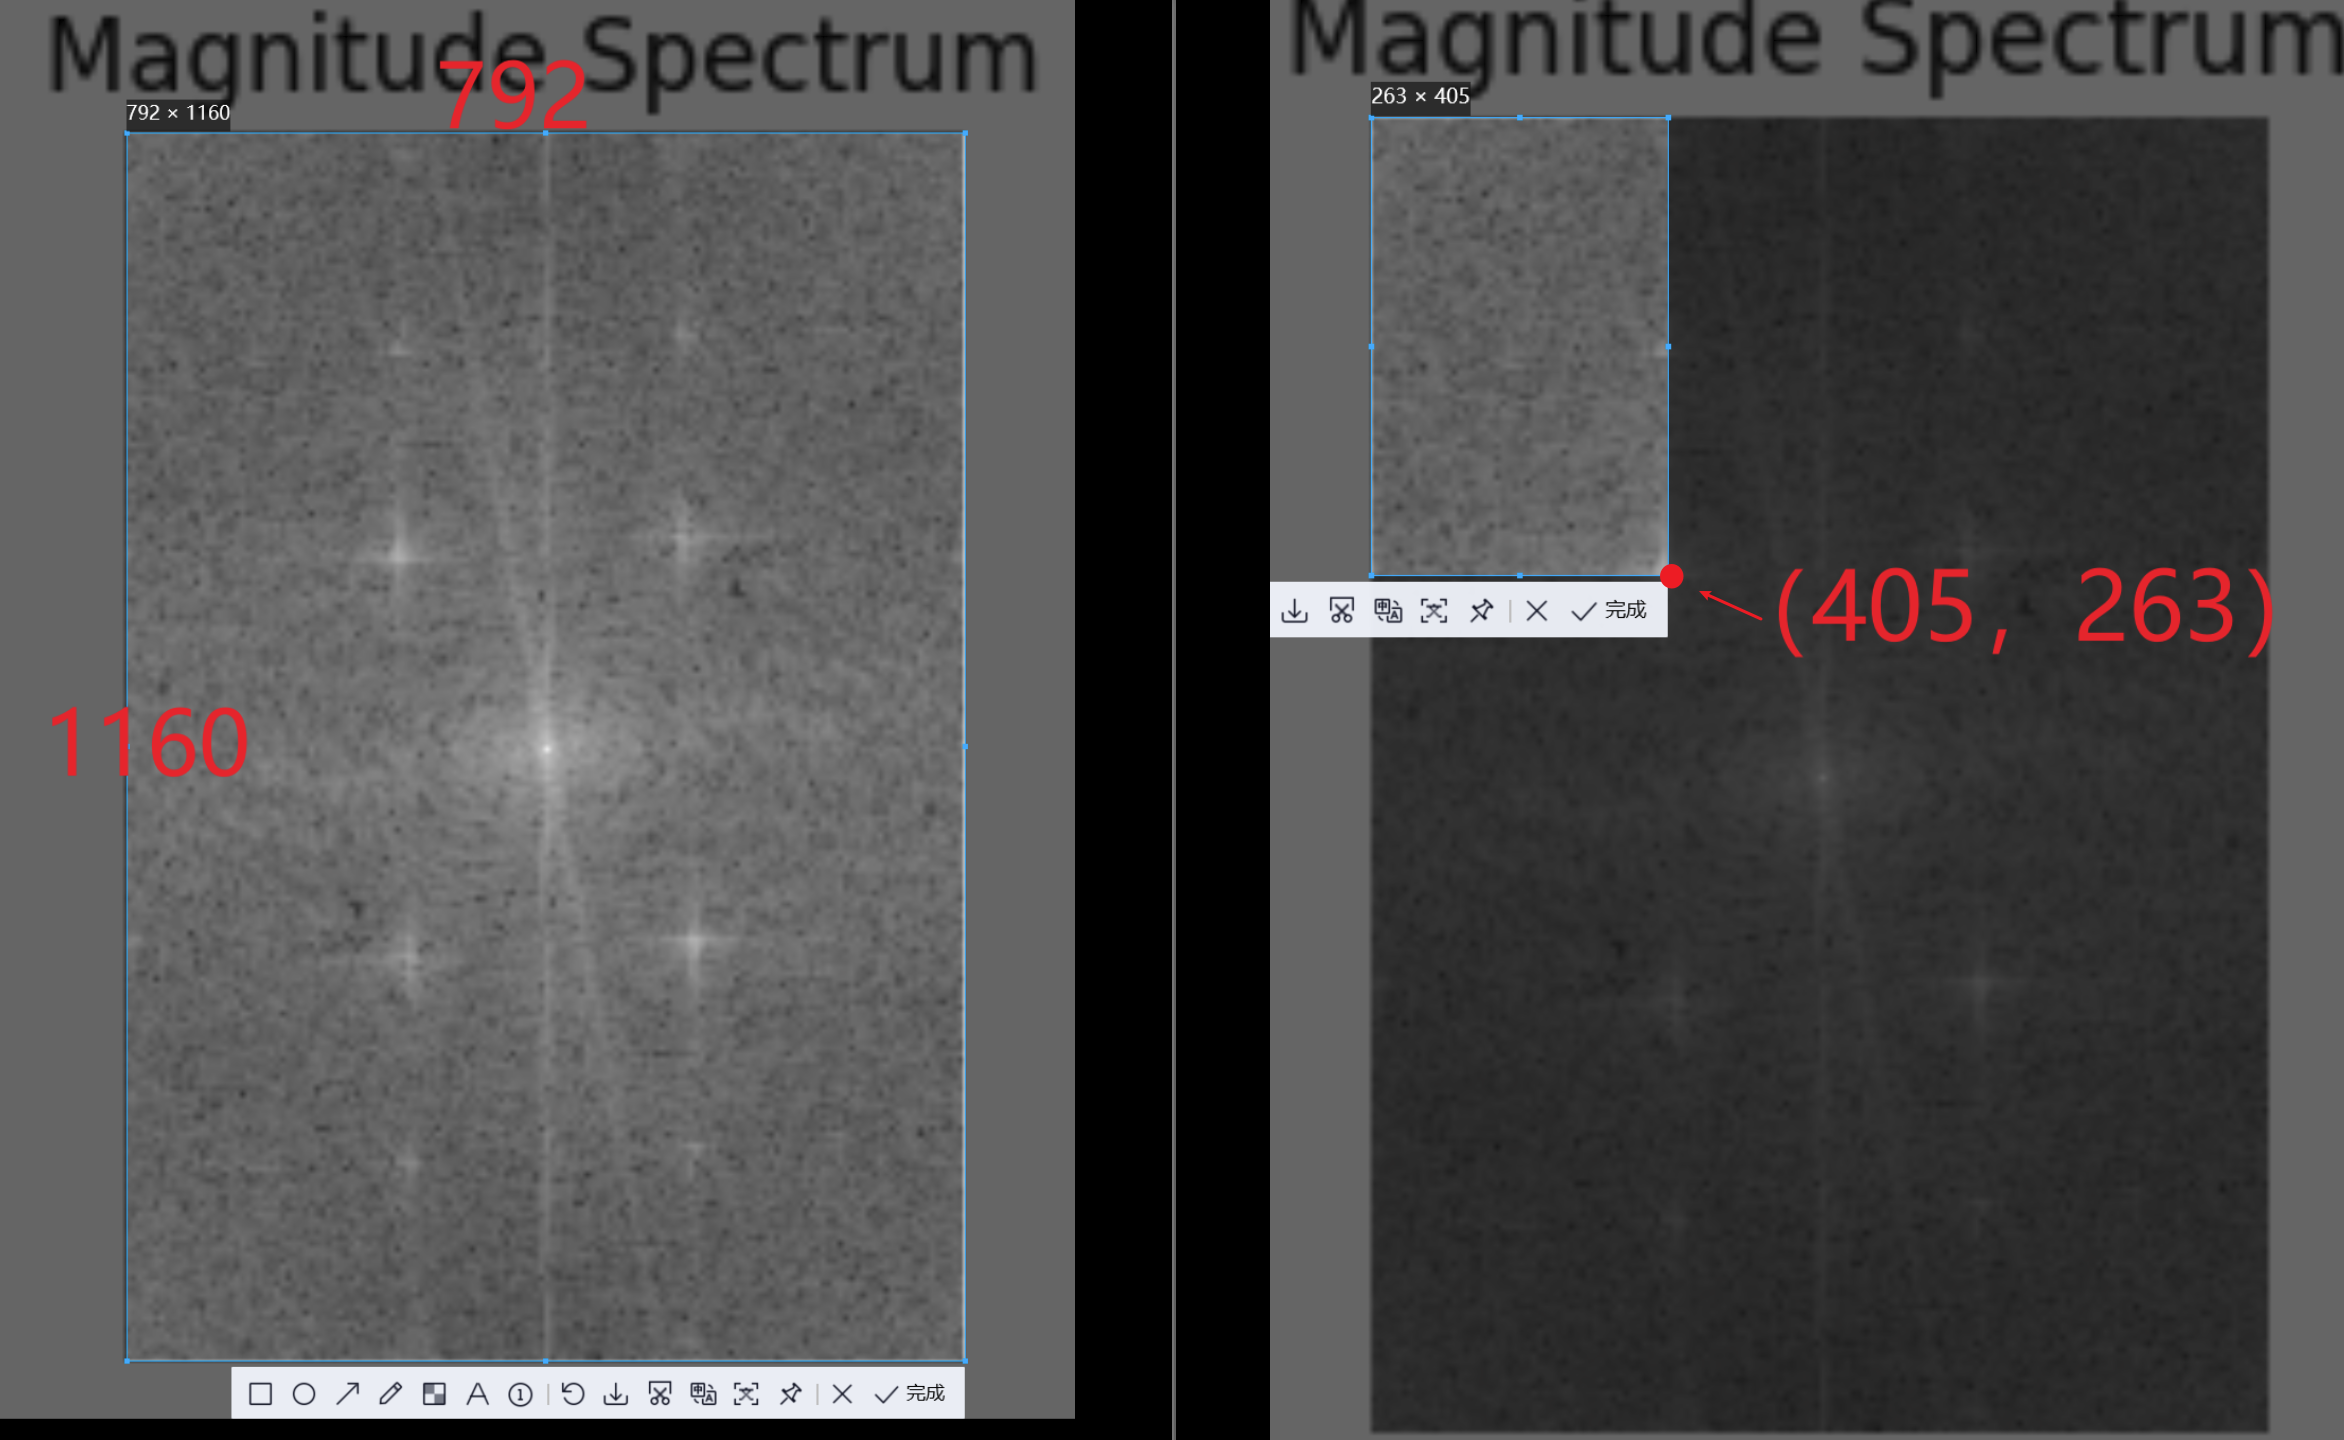
\includegraphics{D:/Tangent/SUSTech/大三下/课程资料/DIP/Lab/lab repo/Lab5/report/assets/image-20240409194142058.png}

Although I have tried to use some image processing methods to find the
position of those bright spots, I failed because there is also a lot of
unstructured bright noise in this spectrum. So even after using some
filtering techniques, it is still hard to determine the exact positions
of those bright spots.

However, the ``snipping method'' seems rough, it works well for this
example.

For the order parameter, I use the default value of 4, which is enough
to filter out the noise. If \texttt{order} is too large, there may exist
ring effect because it behaves more like an ideal filter. If
\texttt{order} is too small, the filtering effect is weak.

Note that I chose the filter shown in Figure todo be real and symmetric,
which is significant if we directly perform filtering solely in the
frequency domain (just as indicated \textbf{on Slide 69 of Lecture 4}).
The filter needs to be symmetric because it corresponds to a real
spatial kernel, and we can only perform convolution for an image of real
value and a kernel of real value. The filter needs to be symmetric
because by doing this, we can ensure the filter is zero-phase and will
not change the fundamental information of an image since the phase of an
image carries its fundamental information.

However, there is an exception. In the previous experiment, we used a
Sobel kernel which is odd-symmetric if zero-padded decently. The
odd-symmetric kernel corresponds to a pure imaginary spectrum, which can
impact the image phase. But this kernel still works well and preserves
the information of the image, so I conclude that if a frequency domain
filter has a spatial domain counterpart that is a kernel too small
(maybe \(3\times 3 \) ?) to carry its own information, it will not harm
the image information even its spectrum is not zero-phase.

\hypertarget{conclusion}{%
\section{Conclusion}\label{conclusion}}

In this lab, we compared the difference between spatial and frequency
domain filtering. Simply put, convolution in the spatial domain is
equivalent to multiplication in the frequency domain. However, in each
domain, we have different methods of designing filters, and in the
frequency domain, we can design powerful filters more easily and
explainably. Like the Butterworth notch filter example, it is hard for
us to find its spatial domain counterpart.

\end{document}
